% Sångtext till VN:s sångbok 2010.

% Denna fil kan användas som sådan, bara verserna,
% namnen och annan rådata behöver bytas ur fälten.
% Tecknet "%" markerar en kommentar som helt och 
% hållet ignoreras av programmet som läser filen.

\beginsong{Skönheten och odjuret}[ 		% Börja sången här
	by={},					% Författare
	sr={Kostervalsen},					% Melodi
	index={Johansson är ful}]						% sångnamn
	

\beginverse*						% Börja vers
Johansson är ful,
han får gömma sig i ett skjul.
Ful är Perssons bror,
Persson själv har förträngt var han bor.
Fulhet gör mig trött,
ge mig snabbt någonting som är sött!
Ge mig punsch,
ett glas med punsch,
nej, en flaska med punsch!
(Å' en kasse bärs.)
\endverse							% Sluta vers



\endsong							% Sluta sång

\begin{figure}[!b]
 \begin{center}
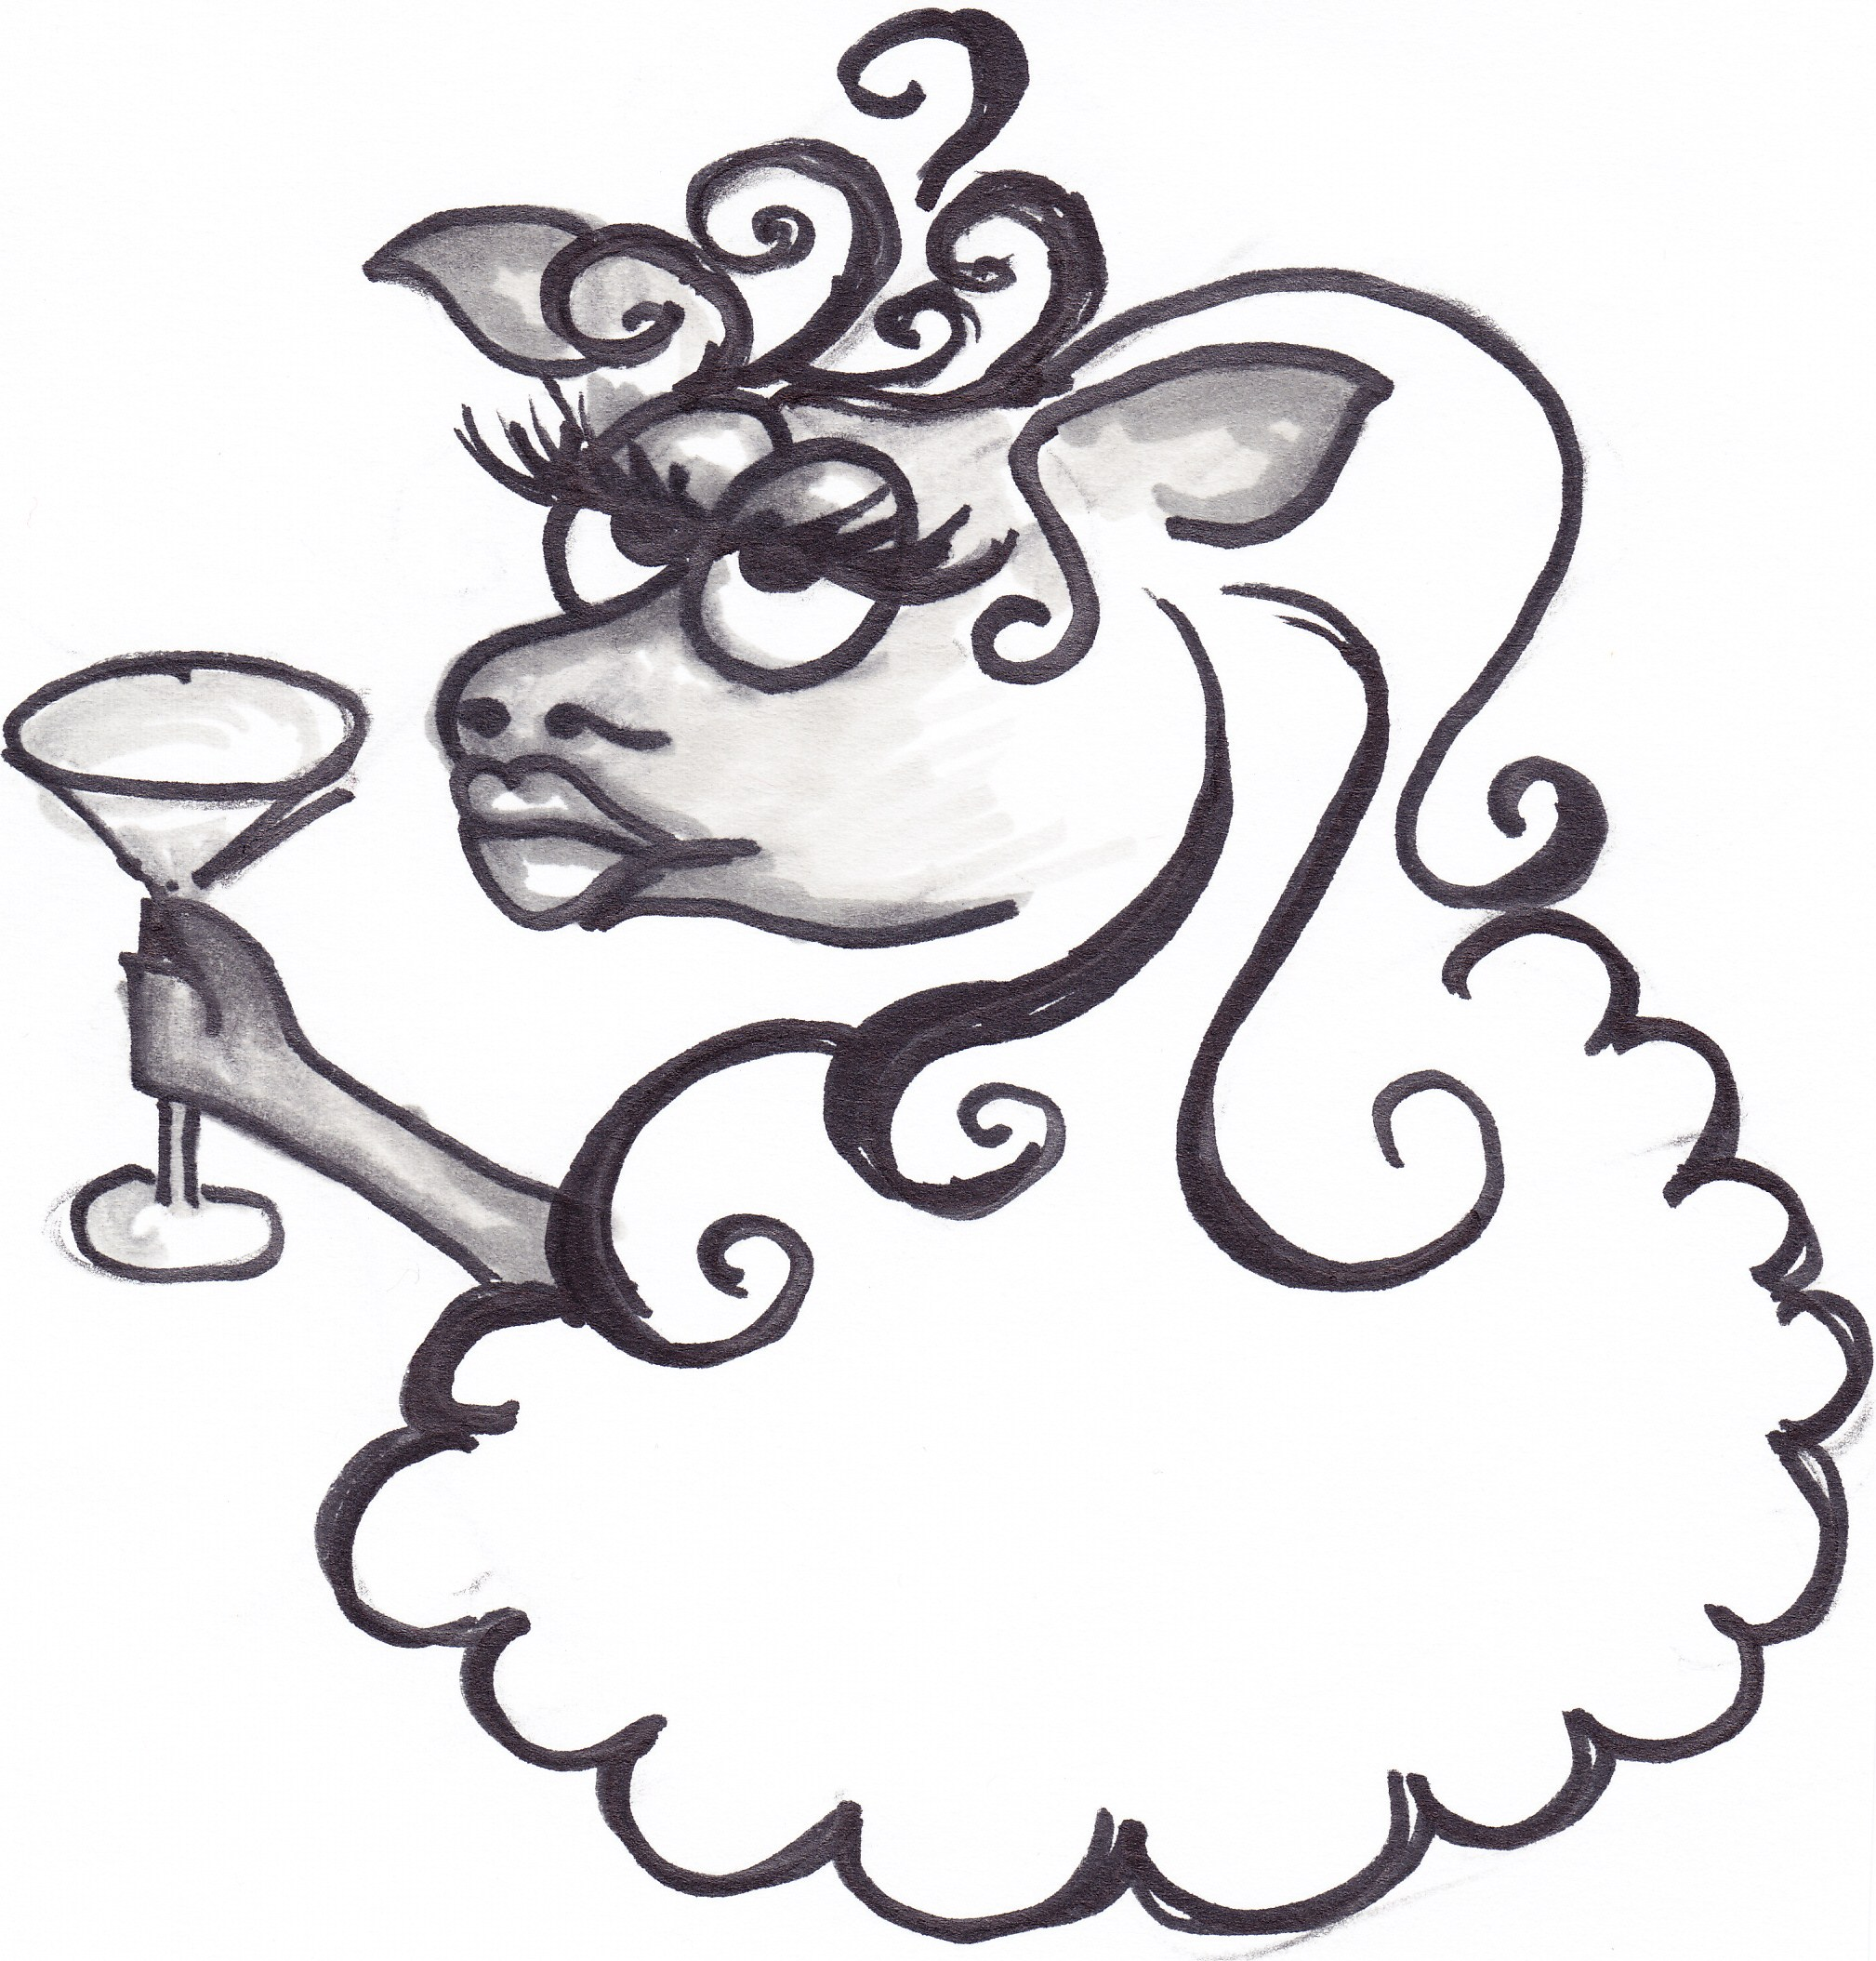
\includegraphics[scale=.2]{../bilder/drickande_far.jpg} 
\end{center}
\end{figure}